\documentclass[xcolor = {svgnames,x11names}]{beamer}

\mode<presentation> {
  \usetheme{Malmoe}
  % ou autre ...

  \setbeamercovered{transparent}
  % ou autre chose (il est également possible de supprimer cette ligne)
}


%\usepackage[english]{babel}
% or autre comme par exemple \usepackage[english]{babel}

%\usepackage[latin1]{inputenc}
% or autre

\usepackage{times}
%\usepackage[T1]{fontenc}
% Or autre. Notez que le codage et la fonte doivent être assortis. Si T1
% ne paraît pas très esthétique, essayer d'effacer la ligne contenant fontenc.

\usepackage{color}
\usepackage{tikz}
\usetikzlibrary{arrows,positioning}
\usepackage{algorithm}
\usepackage{algorithmic}
\usepackage{hyperref}
\usepackage{multimedia}
\usepackage{listings}
\usepackage[utf8]{inputenc}
\usepackage[frenchb]{babel}
\usepackage{aeguill}
\usepackage{import}
%\usepackage{leftidx}
\usepackage{mathtools}

\newcommand\vect[1]{\textbf{#1}}
\newcommand\CS{{\cal C}}
\newcommand\rational{\mathbb{Q}}
\newcommand\real{\mathbb{R}}
\newcommand\Sone{\mathbb{S}^1}
\newcommand\conf{\textbf{q}}
\newcommand\M[2]{\prescript{#1}{}M_{#2}}
\newcommand\x{\vect{x}}
\newcommand\y{\vect{y}}
\newcommand\z{\vect{z}}
\newcommand\WS{{\cal W}}
\newcommand\robot{{\cal R}}
\newcommand\body{{\cal B}}
\newcommand\obst{{\cal O}}
\newcommand\CSobst{\CS_{obst}}
\newcommand\CSfree{\CS_{free}}
\newcommand\sturm{\textbf{sturm}}
\newcommand\var{\textbf{n}_{chsgn}}
\newcommand\nor{\textbf{nr}}
\newcommand\signe{\textbf{signe}}
\newcommand\Kappa{{\cal K}}
\newcommand\calP{{\cal P}}
\newcommand\moment{\vect{M}}
\newcommand\resultante{\vect{R}}
\newcommand\f{\vect{f}}
\newcommand\vel{\vect{v}}
\newcommand\gravity{\vect{g}}
\newcommand\trans{\vect{t}}
\newcommand\rotation{R}
\newcommand\utheta{u_{\theta}}
\newcommand\cinematique{\mathcal{V}}
\newcommand\alcv{{\cal A}}
\newcommand\mloc{{\cal M}_{loc}}
\newcommand\control{\mathbf{u}}
\newcommand\crossprod[1]{\left[{#1}\right]_{\times}}
\newcommand\angularmomentum{\mathbf{L}}
\newcommand\length{\ell}
\newcommand\yaw{\mbox{yaw}}
\definecolor{grey}{rgb}{0.5,0.5,0.5}


\title {Planification de mouvement}

\subtitle{}

\author[]
{Joseph Mirabel}

\institute[CNRS-LAAS] % (facultatif mais généralement nécessaire)
{
  CNRS-LAAS, Toulouse, France
}
\date[] % (facultatif, peut être une abréviation du nom de la conférence)
{}

\begin{document}

\lstset{
breakatwhitespace=true,
%language=C++,
%columns=fullflexible,
%keepspaces=true,
breaklines=true
tabsize=3, 
%showstringspaces=false,
%extendedchars=true
}

\begin{frame}
  \titlepage
\end{frame}

\section{Introduction}
\begin{frame}{Planification de mouvement}
  \tableofcontents[currentsection,currentsubsection]
  % Vous pouvez, si vous le souhaiter ajouter l'option [pausesections]
\end{frame}
\input {introduction}

\section{Cha\^ine cin\'ematique}
\begin{frame}{Planification de mouvement}
  \tableofcontents[currentsection,currentsubsection]
  % Vous pouvez, si vous le souhaiter ajouter l'option [pausesections]
\end{frame}
%\section {Définitions}

%
%  Robot
%

\begin{frame} {Articulations}
  \centerline {
    \parbox {.53\linewidth} {
      \emph{Robot}~: Ensemble de corps rigides li\'ees les uns aux autres par des \textit{articulations}.
      \vskip .5cm
      \pause
      \emph{Transformation}~: une translation $\trans$ et une rotation $\rotation$.
      L'ensemble des transformations forment l'espace $SE(3)$.
      \vskip .5cm
      \pause
      \emph{Articulation}~: transformation $\left( \trans(\conf), \rotation(\conf) \right)$ entre deux repères param\'etr\'es par une ou plusieurs
      variables $\conf \in \real^n$.
    }
    \parbox{.45\linewidth} {
      \centerline {
        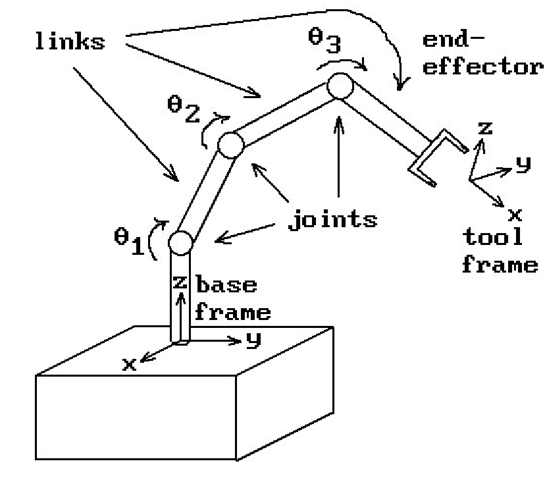
\includegraphics[width=\linewidth]{img/kinematic_chain.png}
      }
    }
  }
\end{frame}

%
%  Articulation
%
\begin{frame} {Articulations: Rotation 1D}
  \centerline {
    \parbox {.53\linewidth} {
      \begin {itemize}
      \item Rotation autour de \z~:
        \begin{eqnarray*}
          \real & \rightarrow & SE(3) \\
          \conf_0 & \rightarrow & (0_{\real^3}, \rotation)
        \end{eqnarray*}
      \end {itemize}
      \vskip .5cm
      \pause
      $$ \rotation=\left(\begin{array}{ccc}\cos \conf_0 & -\sin \conf_0 & 0 \\ \sin \conf_0 & \cos \conf_0 & 0 \\ 0&0&1\end{array}\right)$$
    }
    \parbox{.45\linewidth} {
      \centerline {
        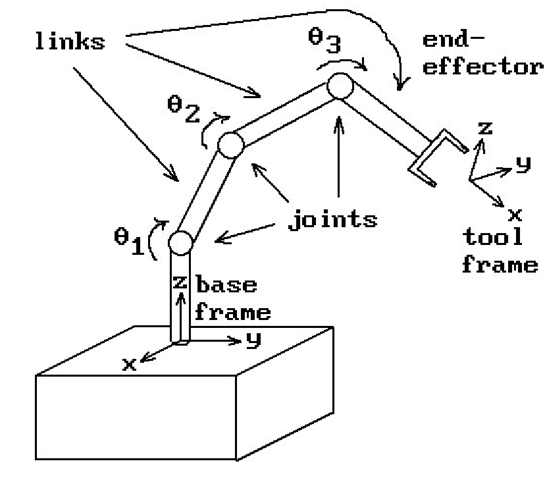
\includegraphics[width=\linewidth]{img/kinematic_chain.png}
      }
    }
  }
\end{frame}

%
%  Articulation
%
\begin{frame} {Articulations: Translation 1D}
  \centerline {
    \parbox {.53\linewidth} {
      \begin {itemize}
      \item Translation selon \x~:
        \begin{eqnarray*}
          \real & \rightarrow & SE(3) \\
          \conf_0 & \rightarrow & (\trans, I_3)
        \end{eqnarray*}
      \end {itemize}
      \vskip .5cm
      \pause
      $$ \trans=\left(\begin{array}{c} \conf_0 \\ 0 \\ 0 \\ \end{array}\right)$$
      $$ I_3=\left(\begin{array}{ccc} 1 & 0 & 0 \\ 0 & 1 & 0 \\ 0&0&1\end{array}\right)$$
    }
    \parbox{.45\linewidth} {
      \centerline {
        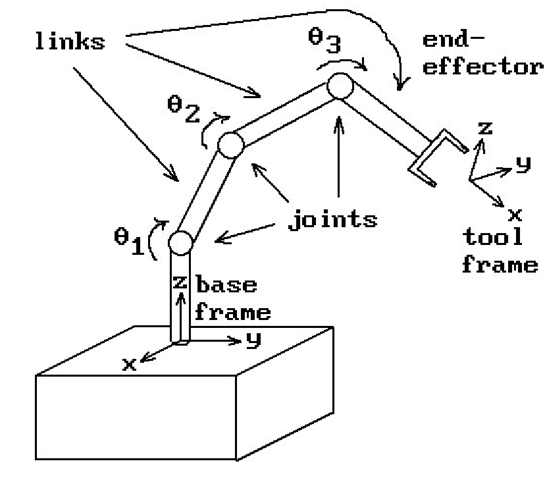
\includegraphics[width=\linewidth]{img/kinematic_chain.png}
      }
    }
  }
\end{frame}

%
%  Articulation
%
\begin{frame} {Articulations: Translation 3D}
  \centerline {
    \parbox {.53\linewidth} {
      \begin {itemize}
      \item Translation~:
        \begin{eqnarray*}
          \real^3 & \rightarrow & SE(3) \\
          \left( \conf_0,\conf_1,\conf_2 \right) & \rightarrow & (\trans, I_3)
        \end{eqnarray*}
      \end {itemize}
      \vskip .5cm
      \pause
      $$ \trans=\left(\begin{array}{c} \conf_0 \\ \conf_1 \\ \conf_2 \\ \end{array}\right)$$
      $$ I_3=\left(\begin{array}{ccc} 1 & 0 & 0 \\ 0 & 1 & 0 \\ 0&0&1\end{array}\right)$$
    }
    \parbox{.45\linewidth} {
      \centerline {
        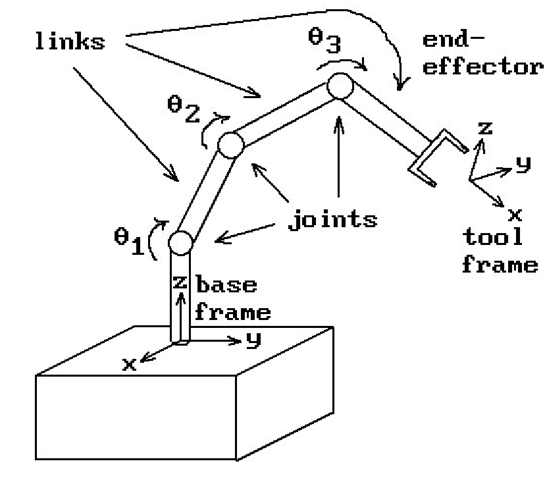
\includegraphics[width=\linewidth]{img/kinematic_chain.png}
      }
    }
  }
\end{frame}

%
%  Articulation
%
\begin{frame} {Articulations: Rotation 3D}
  \centerline {
    \parbox {.54\linewidth} {
      \begin {itemize}
      \item Vecteur de taille 4 unitaire:
        $$\mathbb{S}^4 = \left\{ \conf | \conf\in\real^4, ||\conf||=1 \right\}$$
      \pause
      \item Rotation~:
        \begin{eqnarray*}
           \mathbb{S}^4 & \rightarrow & SE(3) \\
           \conf & \rightarrow & (0_{\real^3}, \rotation(\conf))
        \end{eqnarray*}
      \end {itemize}
      \vskip .5cm
      \pause
      {\tiny
          $$\begin{array}{c}R(\conf)=\\
          \left(\begin{array}{ccc}1 - 2(\conf_2^2 + \conf_3^2) & 2\conf_2\conf_1 - 2\conf_3\conf_0 & 2\conf_3\conf_1 + 2\conf_2\conf_0\\ 2\conf_2\conf_1 + 2\conf_3\conf_0 & 1 - 2(\conf_1^2 + \conf_3^2) & 2\conf_3\conf_2 - 2\conf_1\conf_0\\ 2\conf_3\conf_1 - 2\conf_2\conf_0 & 2\conf_3\conf_2 + 2\conf_1\conf_0 & 1 - 2(\conf_1^2 + \conf_2^2)\end{array}\right)\end{array}$$
          $$\conf_0 + \conf_1 i + \conf_2 j + \conf_3 k\ \mbox{is a quaternion.}$$
      }
    }
    \parbox{.45\linewidth} {
      \centerline {
        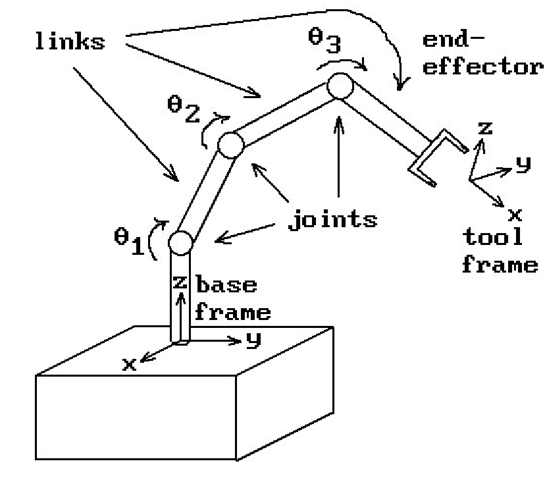
\includegraphics[width=\linewidth]{img/kinematic_chain.png}
      }
    }
  }
\end{frame}

%
%  Quaternions
%
\begin{frame} {Digression: Quaternions}
  \begin{itemize}
    \item Nombres complexes: $i^2 = -1$
    \item Quaternion: extension des nombres complexes
      $$i^2 = j^2 = k^2 = ijk = -1$$
      d'o\`u l'on d\'eduit
      $$ ij=k,\ jk=i,\ ki=j$$
    \item $\conf = \conf_3 + \conf_0 i + \conf_1 j + \conf_2 k $, with $\conf\in\real^4$.
    \item Quaternion unitaire: $\conf_3^2 + \conf_0^2  + \conf_1^2 + \conf_2^2  = 1$.
  \end{itemize}
\end{frame}

%
%  Quaternions
%
\begin{frame} {Digression: Rotation 3D et quaternion unitaire}
  \centerline {
    \parbox{.30\linewidth} {
      \centerline {
        \graphicspath{{./img/}}
        \def\svgwidth{\linewidth}
        \input{img/Angle_axis_vector.pdf_tex}
      }
    }
    \parbox {.68\linewidth} {
      \begin {itemize}
        \item<1-> Rotation identit\'e: $ \conf = \left( 0, 0, 0, 1 \right)$
        \item<2-> Rotation de $\theta$ autour de $\vect{e}$
          $$ \conf = \left( \vect{u}_0, \vect{u}_1, \vect{u}_2, cos(\frac{\theta}{2}) \right)$$
          avec $ \vect{u} = sin(\frac{\theta}{2}) \vect{e}$.
        \item<3->$\conf$ et $-\conf$ repr\'esente la m\^eme rotation.
      \end {itemize}
    }
  }
\end{frame}

%
%  Chaine cinematique
%
\begin{frame} {Cha\^ine cin\'ematique}
  \centerline {
    \parbox {.59\linewidth} {
      \begin {itemize}
        \item Sequence de 3 rotations : $\M{1}{1'}(\conf_1)$,
          $\M{2}{2'}(\conf_2)$ et $\M{3}{3'}(\conf_3)$.
        \item Articulation rigidement li\'ee entre elles : $\M{0}{1}$,
          $\M{1'}{2}$, $\M{2'}{2}$ et $\M{3'}{outil}$.
        \item Configuration du robot: $\conf = \left( \conf_1, \conf_2, \conf_3 \right)$
        \item Calcul de la position de l'outil :
      \end {itemize}
    }
    \parbox{.40\linewidth} {
      \centerline {
        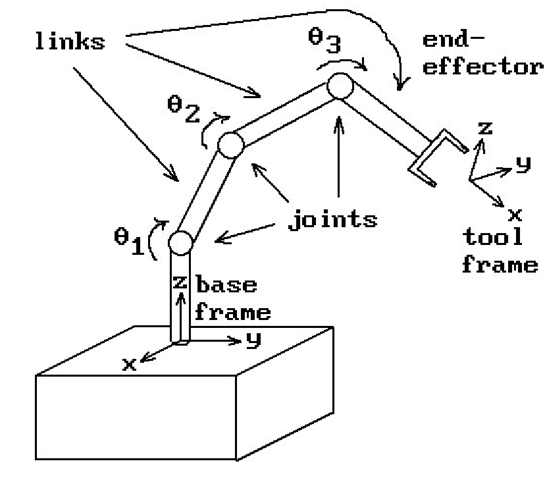
\includegraphics[width=\linewidth]{img/kinematic_chain.png}
      }
    }
  }
  $$
  \M{0}{outil} =
  \M{0}{1}           .
  \M{1}{1'}(\conf_1) .
  \M{1'}{2}          .
  \M{2}{2'}(\conf_2) .
  \M{2'}{3}          .
  \M{3}{3'}(\conf_3) .
  \M{3'}{outil}
  $$
\end{frame}

%
%  Jacobienne
%
\begin{frame} {Cha\^ine cin\'ematique : Jacobienne}
  \centerline {
    \parbox {.59\linewidth} {
      \begin{itemize}
        \item<1-> Contr\^ole du robot via les moteurs: $\conf$
        \item<2-> On veut contr\^oler l'organe terminal: $\M{0}{outil}$
        \item<3-> Relation entre $\dot{\conf}$ et $\vect{V}_{A\in outil / 0}$ ?
        \item<4-> Relation entre $\tau$        et $\vect{F}_{A, outil / 0}$ ?
      \end{itemize}
    }
    \parbox{.40\linewidth} {
      \centerline {
        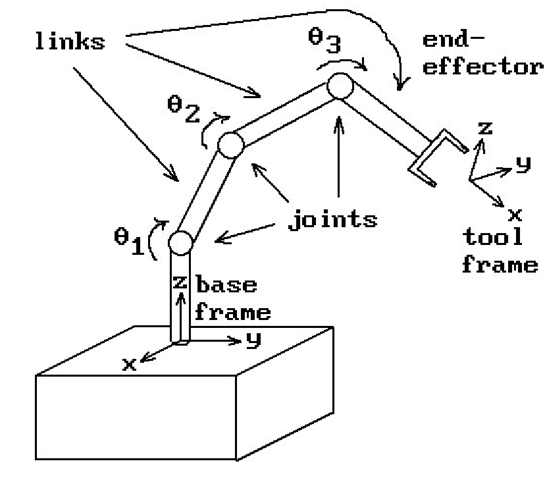
\includegraphics[width=\linewidth]{img/kinematic_chain.png}
      }
    }
  }
\end{frame}

%%%%%%%%%%%%%%%%%%%%%%%%%%%%%%%%%%%%%%%%%%%%%%%%%%%%%%%%%%%%%%%%%%%%%

\begin{frame} {Un cas plus complexe: robot humano\"ide}
  \centerline {
    \parbox{.66\linewidth} {
      Cha\^ine cin\'ematique:
      \vskip .5cm
      \centerline {
        \def\svgwidth {.5\linewidth}
        {\tiny
          \graphicspath{{./figures/}}
          \input {figures/kinematic-chain.pdf_tex}
        }
      }
      \vskip .5cm
      N\'ec\'essit\'e de repr\'esenter un corps flottant.
    }
    \parbox {.33\linewidth} {
      \centerline {
        \includegraphics[width=\linewidth]{figures/hrp2.jpg}
      }
    }
  }
\end{frame}

%
%  Obstacle
%

\begin{frame} {Definitions}

\begin{itemize}
  \item \emph{Espace de travail} dans lequel le robot bouge: $\WS=\real^2$ o\`u $\real^3$
    \pause
  \item Obstacle dans $\WS$: sous-ensemble compact de $\WS$, not\'e $\obst$.
    \pause
  \item Espace des configurations: $\CS$.
    \pause
  \item Position en une configuration $\conf$ d'un point $M\in\body_i$:
    $\x_i(M,\conf)$.
    \pause
  \item Obstacle dans l'espaces des configurations:
    \begin{eqnarray*}
      \CSobst&=\{\conf\in\CS,&\exists i\in\{1,\cdots,m\},\ \exists M\in\body_i,\ \x_i(M,\conf)\in\obst\ \mbox{or}\\
      &&\exists i,j\in\{1,\cdots,m\},\ \exists M_i\in\body_i,\ \exists M_j\in\body_j,\\
    &&\x_i(M_i,\conf)=x_j(M_j,\conf)\}
  \end{eqnarray*}
  \pause
\item Espace des configurations \emph{libres}: $\CSfree = \CS\setminus\CSobst$.
\end{itemize}
\end{frame}

%
%  Motion
%

\begin{frame} {Chemin}
  \begin{itemize}
    \item Chemin:
      \begin{itemize}
        \item fonction continue de $[0,1]$ dans $\CS$.
      \end{itemize}
      \pause
    \item Chemin sans collision:
      \begin{itemize}
        \item fonction continue de $[0,1]$ dans $\CSfree$.
      \end{itemize}
  \end{itemize}
\end{frame}

%
%  Motion
%

\begin{frame}{Probl\'eme de planification de mouvement}
  \begin{itemize}
    \item \'Etant donn\'e un robot, des obstacles ainsi qu'une configuration initial et finale du robot,
      \begin{itemize}
        \item<2-> trouver un chemin sans collision allant de la configuration initiale à la configuration finale.
      \end{itemize}
  \end{itemize}
  \onslide+<3->{
    \begin{itemize}
      \item \'Etant donn\'e un robot, $\obst$, $(\conf_{initiale}, \conf_{finale})\in\CS^2$,
        \begin{itemize}
          \item \onslide+<4-> {trouver $f\in\mathcal{C}^0([0,1], \CSfree)$ telle que $f(0) = \conf_{initiale}$ et $f(1) = \conf_{finale}$.}
        \end{itemize}
    \end{itemize}
  }
\end{frame}


\section{Algorithmes}
\begin{frame}{Planification de mouvement}
  \tableofcontents[currentsection,currentsubsection]
  % Vous pouvez, si vous le souhaiter ajouter l'option [pausesections]
\end{frame}
%\section {Random methods}

%
%  histoire
%

\begin{frame}[<+->]{Un peu d'histoire}
  Les premi\`eres approches sont d\'eterministes :
  \begin{itemize}
    \item discretisation,
      \begin{itemize}
        \item dimensionnalit\'e
      \end{itemize}
    \item diagrammes de Vorono\"i
      \begin{itemize}
        \item dur \`a g\'en\'eraliser pour plus de 2-3 dimensions.
        \item dimensionnalit\'e
      \end{itemize}
    \item décomposition cellulaire
      \begin{itemize}
        \item dur \`a g\'en\'eraliser pour plus de 2-3 dimensions.
        \item dimensionnalit\'e
      \end{itemize}
    \item champs de potentiel
      \begin{itemize}
        \item dur \`a g\'en\'eraliser pour des corps complexes,
        \item sujet au probl\`eme des minimums locaux.
      \end{itemize}
  \end{itemize}
  \onslide+<+->{\'Emergence de m\'ethodes al\'eatoires dans les ann\'ees 1990.}
\end{frame}

%
%  random methods
%

\begin{frame} {M\'ethodes al\'eatoires}
  Principe :
  \begin{itemize}
    \item tirer une configuration al\'eatoire,
      \pause
    \item construire un graphe (carte) dont les noeuds sont des configurations,
      \pause
    \item et dont les ar\^etes sont des interpolations lin\'eaires sans collision.
  \end{itemize}
\end{frame}

%
%  La méthode du réseau aléatoire
%

\begin{frame} {Probabilistic roadmap (PRM) 1994}
\centerline {
  \includegraphics[width=.8\linewidth]{figures/PRM1.pdf}
}
\end{frame}

\begin{frame} {Probabilistic roadmap (PRM) 1994}
\centerline {
  \includegraphics[width=.8\linewidth]{figures/PRM2.pdf}
}
\end{frame}

\begin{frame} {Probabilistic roadmap (PRM) 1994}
\centerline {
  \includegraphics[width=.8\linewidth]{figures/PRM3.pdf}
}
\end{frame}

\begin{frame} {Probabilistic roadmap (PRM) 1994}
\centerline {
  \includegraphics[width=.8\linewidth]{figures/PRM4.pdf}
}
\end{frame}

\begin{frame} {Probabilistic roadmap (PRM) 1994}
\centerline {
  \includegraphics[width=.8\linewidth]{figures/PRM5.pdf}
}
\end{frame}

\begin{frame} {Probabilistic roadmap (PRM) 1994}
\centerline {
  \includegraphics[width=.8\linewidth]{figures/PRM6.pdf}
}
\end{frame}

\begin{frame} {Probabilistic roadmap (PRM) 1994}
\centerline {
  \includegraphics[width=.8\linewidth]{figures/PRM7.pdf}
}
\end{frame}

\begin{frame} {Probabilistic roadmap (PRM) 1994}
\centerline {
  \includegraphics[width=.8\linewidth]{figures/PRM8.pdf}
}
\end{frame}

\begin{frame} {Probabilistic roadmap (PRM) 1994}
\centerline {
  \includegraphics[width=.8\linewidth]{figures/PRM9.pdf}
}
\end{frame}

\begin{frame} {Probabilistic roadmap (PRM) 1994}
\centerline {
  \includegraphics[width=.8\linewidth]{figures/PRM10.pdf}
}
\end{frame}

\begin{frame} {Probabilistic roadmap (PRM) 1994}
\centerline {
  \includegraphics[width=.8\linewidth]{figures/PRM11.pdf}
}
\end{frame}

\begin{frame} {Probabilistic roadmap (PRM) 1994}
\centerline {
  \includegraphics[width=.8\linewidth]{figures/PRM12.pdf}
}
\end{frame}

\begin{frame} {Probabilistic roadmap (PRM) 1994}
\centerline {
  \includegraphics[width=.8\linewidth]{figures/PRM13.pdf}
}
\end{frame}

\begin{frame} {Probabilistic roadmap (PRM) 1994}
\centerline {
  \includegraphics[width=.8\linewidth]{figures/PRM14.pdf}
}
\end{frame}

\begin{frame} {Probabilistic roadmap (PRM) 1994}
\centerline {
  \includegraphics[width=.8\linewidth]{figures/PRM15.pdf}
}
\end{frame}

\begin{frame} {Probabilistic roadmap (PRM) 1994}
\centerline {
  \includegraphics[width=.8\linewidth]{figures/PRM16.pdf}
}
\end{frame}

\begin{frame} {Probabilistic roadmap (PRM) 1994}
\centerline {
  \includegraphics[width=.8\linewidth]{figures/PRM17.pdf}
}
\end{frame}

\begin{frame} {Probabilistic roadmap (PRM) 1994}
\centerline {
  \includegraphics[width=.8\linewidth]{figures/PRM18.pdf}
}
\end{frame}

\begin{frame} {Probabilistic roadmap (PRM)}
  \begin{itemize}
  \item Beaucoup de noeuds inutiles sont cr\'e\'es,
    \begin{itemize}
    \item cela augmente le co\^ut de connexion de nouveaux noeuds \'a la carte courrante.
    \end{itemize}
  \item Am\'elioration: Visibility-based PRM
    \begin{itemize}
    \item Seul les noeuds \textit{int\'eressants} sont gard\'es.
    \end{itemize}
  \end{itemize}
\end{frame}


%
%  Visibility-based probabilistic roadmap
%
\begin{frame} {Visibility-based probabilistic roadmap (Visi-PRM) 1999}
\centerline {
  \includegraphics[width=.8\linewidth]{figures/VPRM1.pdf}
}
\end{frame}

\begin{frame} {Visibility-based probabilistic roadmap (Visi-PRM) 1999}
\centerline {
  \includegraphics[width=.8\linewidth]{figures/VPRM2.pdf}
}
\end{frame}

\begin{frame} {Visibility-based probabilistic roadmap (Visi-PRM) 1999}
\centerline {
  \includegraphics[width=.8\linewidth]{figures/VPRM3.pdf}
}
\end{frame}

\begin{frame} {Visibility-based probabilistic roadmap (Visi-PRM) 1999}
\centerline {
  \includegraphics[width=.8\linewidth]{figures/VPRM4.pdf}
}
\end{frame}

\begin{frame} {Visibility-based probabilistic roadmap (Visi-PRM) 1999}
\centerline {
  \includegraphics[width=.8\linewidth]{figures/VPRM5.pdf}
}
\end{frame}

\begin{frame} {Visibility-based probabilistic roadmap (Visi-PRM) 1999}
\centerline {
  \includegraphics[width=.8\linewidth]{figures/VPRM6.pdf}
}
\end{frame}

\begin{frame} {Visibility-based probabilistic roadmap (Visi-PRM) 1999}
\centerline {
  \includegraphics[width=.8\linewidth]{figures/VPRM7.pdf}
}
\end{frame}

\begin{frame} {Visibility-based probabilistic roadmap (Visi-PRM) 1999}
\centerline {
  \includegraphics[width=.8\linewidth]{figures/VPRM8.pdf}
}
\end{frame}

\begin{frame} {Visibility-based probabilistic roadmap (Visi-PRM) 1999}
\centerline {
  \includegraphics[width=.8\linewidth]{figures/VPRM9.pdf}
}
\end{frame}

\begin{frame} {Visibility-based probabilistic roadmap (Visi-PRM) 1999}
\centerline {
  \includegraphics[width=.8\linewidth]{figures/VPRM10.pdf}
}
\end{frame}

\begin{frame} {Visibility-based probabilistic roadmap (Visi-PRM) 1999}
\centerline {
  \includegraphics[width=.8\linewidth]{figures/VPRM11.pdf}
}
\end{frame}

\begin{frame} {Visibility-based probabilistic roadmap (Visi-PRM) 1999}
\centerline {
  \includegraphics[width=.8\linewidth]{figures/VPRM12.pdf}
}
\end{frame}

\begin{frame} {Visibility-based probabilistic roadmap (Visi-PRM) 1999}
\centerline {
  \includegraphics[width=.8\linewidth]{figures/VPRM13.pdf}
}
\end{frame}

\begin{frame} {Visibility-based probabilistic roadmap (Visi-PRM) 1999}
\centerline {
  \includegraphics[width=.8\linewidth]{figures/VPRM14.pdf}
}
\end{frame}

\begin{frame} {Visibility-based probabilistic roadmap (Visi-PRM) 1999}
\centerline {
  \includegraphics[width=.8\linewidth]{figures/VPRM15.pdf}
}
\end{frame}

%
%  La méthode des arbres aléatoires d'exploration rapide.
%

\begin{frame} {Rapidly exploring Random Tree (RRT) 2000}
\centerline {
  \includegraphics[width=.8\linewidth]{figures/RRT1.pdf}
}
\end{frame}

\begin{frame} {Rapidly exploring Random Tree (RRT) 2000}
\centerline {
  \includegraphics[width=.8\linewidth]{figures/RRT2.pdf}
}
\end{frame}

\begin{frame} {Rapidly exploring Random Tree (RRT) 2000}
\centerline {
  \includegraphics[width=.8\linewidth]{figures/RRT3.pdf}
}
\end{frame}

\begin{frame} {Rapidly exploring Random Tree (RRT) 2000}
\centerline {
  \includegraphics[width=.8\linewidth]{figures/RRT4.pdf}
}
\end{frame}

\begin{frame} {Rapidly exploring Random Tree (RRT) 2000}
\centerline {
  \includegraphics[width=.8\linewidth]{figures/RRT5.pdf}
}
\end{frame}

\begin{frame} {Rapidly exploring Random Tree (RRT) 2000}
\centerline {
  \includegraphics[width=.8\linewidth]{figures/RRT6.pdf}
}
\end{frame}

\begin{frame} {Rapidly exploring Random Tree (RRT) 2000}
\centerline {
  \includegraphics[width=.8\linewidth]{figures/RRT7.pdf}
}
\end{frame}

\begin{frame} {Rapidly exploring Random Tree (RRT) 2000}
\centerline {
  \includegraphics[width=.8\linewidth]{figures/RRT8.pdf}
}
\end{frame}

\begin{frame} {Rapidly exploring Random Tree (RRT) 2000}
\centerline {
  \includegraphics[width=.8\linewidth]{figures/RRT9.pdf}
}
\end{frame}

\begin{frame} {Rapidly exploring Random Tree (RRT) 2000}
\centerline {
  \includegraphics[width=.8\linewidth]{figures/RRT10.pdf}
}
\end{frame}

\begin{frame} {Rapidly exploring Random Tree (RRT) 2000}
\centerline {
  \includegraphics[width=.8\linewidth]{figures/RRT11.pdf}
}
\end{frame}

\begin{frame} {Rapidly exploring Random Tree (RRT) 2000}
\centerline {
  \includegraphics[width=.8\linewidth]{figures/RRT12.pdf}
}
\end{frame}

\begin{frame} {Rapidly exploring Random Tree (RRT) 2000}
\centerline {
  \includegraphics[width=.8\linewidth]{figures/RRT13.pdf}
}
\end{frame}

\begin{frame} {Rapidly exploring Random Tree (RRT) 2000}
\centerline {
  \includegraphics[width=.8\linewidth]{figures/RRT14.pdf}
}
\end{frame}

\begin{frame} {Rapidly exploring Random Tree (RRT) 2000}
\centerline {
  \includegraphics[width=.8\linewidth]{figures/RRT15.pdf}
}
\end{frame}

\begin{frame} {Rapidly exploring Random Tree (RRT) 2000}
\centerline {
  \includegraphics[width=.8\linewidth]{figures/RRT16.pdf}
}
\end{frame}

\begin{frame} {Rapidly exploring Random Tree (RRT) 2000}
\centerline {
  \includegraphics[width=.8\linewidth]{figures/RRT17.pdf}
}
\end{frame}

\begin{frame} {Rapidly exploring Random Tree (RRT) 2000}
\centerline {
  \includegraphics[width=.8\linewidth]{figures/RRT18.pdf}
}
\end{frame}

\begin{frame} {Rapidly exploring Random Tree (RRT) 2000}
\centerline {
  \includegraphics[width=.8\linewidth]{figures/RRT19.pdf}
}
\end{frame}

\begin{frame} {Rapidly exploring Random Tree (RRT) 2000}
\centerline {
  \includegraphics[width=.8\linewidth]{figures/RRT20.pdf}
}
\end{frame}

%
% random methods
%

\begin{frame} {M\'ethodes al\'eatoires}
  \begin{itemize}
  \item Avantages:
    \begin{itemize}
    \item pas de calcul explicites de l'espace des configurations libres,
    \item facile \'a impl\'ementer,
    \item robuste.
    \end{itemize}
    \pause
  \item Inconv\'enients:
    \begin{itemize}
    \item pas de compl\'etude, seulement une compl\'etude en probabilit\'e.
    \item difficile de trouver un passage \'etroit.
    \end{itemize}
    \pause
  \item Op\'erations requises~:
    \begin{itemize}
    \item test de collisions
      \begin{itemize}
      \item pour des configurations (statique),
      \item pour des chemins (dynamique)
      \end{itemize}
    \end{itemize}
  \end{itemize}
\end{frame}


\section{Planification sous contraintes}
\begin{frame}{Planification de mouvement}
  \tableofcontents[currentsection,currentsubsection]
  % Vous pouvez, si vous le souhaiter ajouter l'option [pausesections]
\end{frame}
% a. présentation du cadre
%   - cas d'usage
%   - quelques définitions
%   - quelques fonctions exemples (position, orientation, COM)
% b. pour les configurations
%   - méthode exacte.
%   - méthode iterative (Newton-Raphson, conditions KKT pour les limites articulaires).
%   - comparaisons des méthodes.
% c. pour les trajectoires (seulement mettre en évidence le problème)

\begin{frame} {Motivations}
  \begin{itemize}
    \item Comment g\'en\'erer une configuration satisfaisant des crit\`eres g\'eom\'etriques ?
      \begin{itemize}
        \item position,
        \item orientation,
        \item centre de masse,
        \item visibilit\'e,
        \item \ldots
      \end{itemize}
      \pause
    \item Interpolation lin\'eraire dans $\CS$:
      \begin{itemize}
        \item courbe non lin\'eraire dans $\WS$
      \end{itemize}
      \pause
  \end{itemize}
\end{frame}

\begin{frame}[<+->]{D\'efinition}
  \emph{Contrainte} : une equation de la forme $$f(q) = 0$$
  \begin{itemize}
    \item<2-> $f \in \mathcal{C}^1(\CS, \real^m)$,
    \item<3-> $m$ est la dimension de la contrainte.
  \end{itemize}

  \onslide+<4->{
    Quelques exemples :
    \begin{itemize}
      \item<5-> position,
      \item<6-> centre de masse,
      \item<7-> orientation.
    \end{itemize}
  }
\end{frame}

\begin{frame}[<+->]{R\'esolution exacte}
  \begin{itemize}
    \item donne l'ensemble des solutions d'une contrainte : ${ q\in\CS, f(q) = 0}$,
    \item possible pour certaines contraintes mais :
      \begin{itemize}
        \item sp\'ecifique \`a chaque cas,
        \item complexes \`a impl\'ementer,
        \item difficile, voire impossible \`a combiner.
      \end{itemize}
  \end{itemize}
\end{frame}

\begin{frame}[<+->]{R\'esolution num\'erique}
  \emph{M\'ethode it\'erative}
  \begin{itemize}
    \item si $ || f(\conf_n) || < \epsilon $ alors $\conf_n$ est une solution,
    \item calcul de la d\'eriv\'ee de $f$ :
      $$J = \frac{\partial f}{\partial \conf}$$
    \item calcul de $\conf_{n+1}$ avec une approximation
      \begin{itemize}
        \item du 1er ordre
          $$\conf_{n+1} = \conf_n - \alpha \left( \frac{||f(\conf_n)||^2}{2 ||J^T f(\conf_n)||^2} \right) J^{T} f(\conf_n), \alpha\in]0,1] $$
        \item du 2nd ordre: $J^{\dagger}$ est la pseudo-inverse de $J$
          $$\conf_{n+1} = \conf_n - \alpha J^{\dagger} f(\conf_n), \alpha\in]0,1] $$
      \end{itemize}
  \end{itemize}
\end{frame}

\begin{frame}[<+->]{Digression: pseudo-inverse}
  Soit $J\in\mathcal{M}_{m,n}(\real), n \ge m$ et soit le probl\`eme 
  $J x = b$.

  \begin{itemize}
    \item $x^* = J^{\dagger} b$ est la solution de norme minimale.
    \item la matrice $I_n - J^\dagger J$ est un projecteur sur le noyau de $J$.
    \item l'ensemble des solutions est $\left\{ x^* + (I_n - J^\dagger J) u, u\in\real^n \right\}$.
  \end{itemize}
\end{frame}

%\begin{frame}[<+->]{Digression: espace null (noyau) d'une matrice}
%  Soit $J\in\mathcal{M}_{n,m}(\real), n \ge m$.
%  La pseudo-inverse $J^{\dagger}$ de $J$ est l'unique matrice qui v\'erifie.
%  alors $J$
%%utilisation de la d\'ecomposition en valeur singuli\`ere (SVD):
%\end{frame}


\section{D\'etection de collision}
\begin{frame}{Planification de mouvement}
  \tableofcontents[currentsection,currentsubsection]
  % Vous pouvez, si vous le souhaiter ajouter l'option [pausesections]
\end{frame}
%\section {Collision tests}

%
%  Collision tests
%
\begin{frame} {Test de collision}
  \begin{itemize}
    \item Probl\`eme: \'etant donn\'e
      \begin{itemize}
        \item deux ensembles rigides de triangles,
        \item la position relative d'un ensemble par rapport \'a l'autre,
      \end{itemize}
      d\'eterminer si l'intersection entre les ensembles est vide.
  \end{itemize}
\end{frame}

%
%  Hierarchy of bounding volumes
%
\begin{frame} {Hi\'erarchie de volumes englobants}
  \begin{itemize}
  \item Arbre binaire de volumes englobants tel que :
    \begin{itemize}
    \item chaque noeud a deux enfants,
    \item les feuilles sont les triangles.
    \end{itemize}
  \end{itemize}
  \only<1>{ \centerline { \includegraphics[width=.8\linewidth]{figures/bvh1.pdf} } }
  \only<2>{ \centerline { \includegraphics[width=.8\linewidth]{figures/bvh2.pdf} } }
  \only<3>{ \centerline { \includegraphics[width=.8\linewidth]{figures/bvh3.pdf} } }
  \only<4>{ \centerline { \includegraphics[width=.8\linewidth]{figures/bvh4.pdf} } }
  \only<5>{ \centerline { \includegraphics[width=.8\linewidth]{figures/bvh5.pdf} } }
  \only<6>{ \centerline { \includegraphics[width=.8\linewidth]{figures/bvh6.pdf} } }
  \only<7>{ \centerline { \includegraphics[width=.8\linewidth]{figures/bvh7.pdf} } }
  \only<8>{ \centerline { \includegraphics[width=.8\linewidth]{figures/bvh8.pdf} } }
  \only<9>{ \centerline { \includegraphics[width=.8\linewidth]{figures/bvh9.pdf} } }
\end{frame}

%
%  Collision tests for configurations
%

\begin{frame} {Test de collision pour des configurations}
  \begin{itemize}
    \item Algorithme
      \begin{itemize}
        \item si les \'el\'ements de la paire sont des feuilles, tester les triangles
        \item si la paire de volume englobant (VE) courante, arr\^eter l'exploration du sous-arbre
        \item d\'eterminer le VE \'a \emph{casser} en deux.
        \item tester r\'ecursivement le VE non \emph{cass\'e} avec les deux fils de l'autre.
      \end{itemize}
      \only<1>{\centerline { \includegraphics[width=.8\linewidth]{figures/collision-test1.pdf} } }
      \only<2>{\centerline { \includegraphics[width=.8\linewidth]{figures/collision-test2.pdf} } }
      \only<3>{\centerline { \includegraphics[width=.8\linewidth]{figures/collision-test3.pdf} } }
  \end{itemize}

\end{frame}

%
%  Collision tests for configurations
%

\begin{frame} {GJK: Gilbert-Johnson-Keerthi}
  \begin{itemize}
    \item Test de collision entre deux ensembles \emph{convexes}.
    \item<2> Point support :
      \onslide+<2>{ \centerline { \includegraphics[width=.8\linewidth]{img/gjk/support.jpeg} } }
  \end{itemize}
\end{frame}

\begin{frame} {GJK: Gilbert-Johnson-Keerthi}
  \begin{itemize}
    \item<1> Somme de Minkowski :
      \only<1>{ \centerline { \includegraphics[width=.8\linewidth]{img/gjk/minkowski-sum.jpeg} } }
    \item<2> Diff\'erence de Minkowski :
      \only<2>{ \centerline { \includegraphics[width=.8\linewidth]{img/gjk/minkowski-diff.jpeg} } }
  \end{itemize}
\end{frame}

\begin{frame} {GJK: Gilbert-Johnson-Keerthi}
  \centerline{ \includegraphics[width=.6\linewidth]{img/gjk/gjk.jpeg} }
\end{frame}


\end{document}
